\documentclass{article}
\usepackage[utf8]{inputenc}
\usepackage[T1]{fontenc}
\usepackage{amsmath}
\usepackage{amsfonts}
\usepackage{amssymb}
\usepackage{pgfplots}
\pgfplotsset{compat=1.18} % Required for pgfplots
\usepackage{geometry}
\geometry{a4paper, margin=1in}
\usepackage{enumitem} % For custom list environments

% Custom command for step-by-step solutions
\newlist{steps}{enumerate}{1}
\setlist[steps]{label=\textbf{Step \arabic*:}, ref=Step \arabic*}

\title{Lesson: Solving Linear Equations and Their Graphical Representation}
\author{Academic LaTeX Expert}
\date{\today}

\begin{document}

\maketitle

\section*{Introduction to Linear Equations}

Welcome to this lesson on linear equations! In Grade 10 algebra, understanding linear equations is fundamental. A linear equation is an algebraic equation in which each term has an exponent of 1, and when graphed, it forms a straight line. They are incredibly useful for modeling real-world situations, from calculating distances and speeds to determining costs and profits.

Our goal when solving a linear equation in one variable is to find the value of the variable that makes the equation true. This often involves isolating the variable on one side of the equation using inverse operations. For linear equations in two variables, we can represent their relationship visually on a coordinate plane.

\section*{Concept Explanation: What is a Linear Equation?}

A linear equation in one variable can generally be written in the form $ax + b = c$, where $a$, $b$, and $c$ are real numbers, and $a \neq 0$. The variable is $x$.

\begin{itemize}
    \item \textbf{Solving:} To solve for $x$, we use inverse operations:
    \begin{enumerate}
        \item Add or subtract terms to get all terms with the variable on one side and constant terms on the other.
        \item Multiply or divide to isolate the variable.
    \end{enumerate}
    \item \textbf{Linear Equations in Two Variables:} An equation like $y = mx + b$ (slope-intercept form) or $Ax + By = C$ (standard form) represents a linear relationship between two variables, typically $x$ and $y$. When plotted on a Cartesian coordinate system, all points $(x, y)$ that satisfy the equation lie on a straight line.
\end{itemize}

Let's work through an example that combines solving a linear equation with understanding its graphical representation.

\section*{Worked Example: The Rectangular Garden}

\textbf{Problem:} A rectangular garden has a perimeter of 40 meters. The length of the garden is 3 meters more than twice its width. Find the dimensions (length and width) of the garden. Then, consider the relationship between the length and width, and visualize it graphically.

\begin{steps}
    \item \textbf{Define Variables:}
    Let $w$ be the width of the garden in meters.
    Let $l$ be the length of the garden in meters.

    \item \textbf{Formulate Equations from the Problem Statement:}
    We are given two pieces of information:
    \begin{itemize}
        \item The perimeter is 40 meters: $P = 2l + 2w$. So, $40 = 2l + 2w$.
        \item The length is 3 meters more than twice its width: $l = 2w + 3$.
    \end{itemize}

    \item \textbf{Substitute and Solve for One Variable:}
    We have a system of two linear equations. We can use substitution. Substitute the expression for $l$ from the second equation into the first equation:
    $40 = 2(2w + 3) + 2w$

    Now, solve for $w$:
    $40 = 4w + 6 + 2w$
    $40 = 6w + 6$
    Subtract 6 from both sides:
    $40 - 6 = 6w$
    $34 = 6w$
    Divide by 6:
    $w = \frac{34}{6} = \frac{17}{3}$ meters

    \item \textbf{Solve for the Other Variable:}
    Now that we have $w$, substitute its value back into the equation for $l$:
    $l = 2w + 3$
    $l = 2\left(\frac{17}{3}\right) + 3$
    $l = \frac{34}{3} + 3$
    To add, find a common denominator:
    $l = \frac{34}{3} + \frac{9}{3}$
    $l = \frac{43}{3}$ meters

    \item \textbf{State the Dimensions:}
    The width of the garden is $\frac{17}{3}$ meters (approximately 5.67 m).
    The length of the garden is $\frac{43}{3}$ meters (approximately 14.33 m).

    \item \textbf{Graphical Representation of the Relationship:}
    The relationship between the length and width is given by $l = 2w + 3$. We can visualize this as a linear equation in two variables. If we let $w$ be represented by the $x$-axis and $l$ by the $y$-axis, the equation becomes $y = 2x + 3$. This is a straight line with a slope of 2 and a $y$-intercept of 3.

    The graph below shows this relationship. Note that in the context of a garden's dimensions, $w$ and $l$ must be positive, so we are primarily interested in the first quadrant. The specific dimensions we found, $w=\frac{17}{3}$ and $l=\frac{43}{3}$, would be a single point on this line.

    \begin{figure}[htbp]htbp]
        \centering
        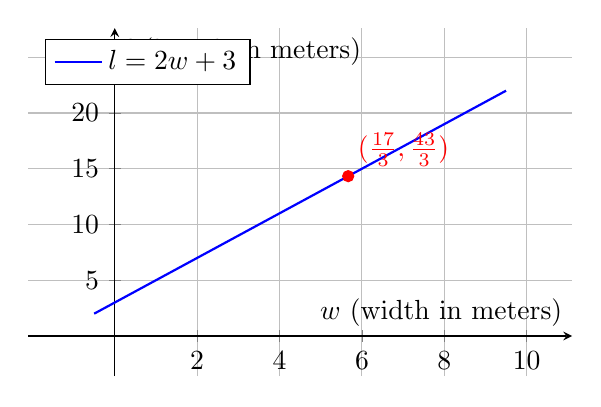
\begin{tikzpicture}
            \begin{axis}[
                axis lines=middle,
                enlargelimits,
                width=0.7\textwidth,
                height=6cm,
                xlabel=$w$ (width in meters),
                ylabel=$l$ (length in meters),
                xmin=-1, xmax=10,
                ymin=-1, ymax=25,
                grid=both,
                xtick={0,2,4,6,8,10},
                ytick={0,5,10,15,20,25},
                legend pos=north west
            ]
            \addplot[domain=-0.5:9.5, samples=100, blue, thick]{2*x+3};
            \addlegendentry{$l=2w+3$}
            % Mark the specific solution point
            \addplot[only marks, mark=*, red, mark size=2pt] coordinates {(17/3, 43/3)};
            \node[above right, red] at (axis cs: 17/3, 43/3) {($\frac{17}{3}, \frac{43}{3}$)};
            \end{axis}
        \end{tikzpicture}
        \caption{Graph of the relationship between length ($l$) and width ($w$) for $l=2w+3$. The red point indicates the specific dimensions of the garden from the problem.}
        \label{fig:length_width_plot}
    \end{figure}
\end{steps}

\section*{Exercises}

Now it's your turn to practice! These exercises are designed to test your understanding at different levels.

\subsection*{Level 1: Basic Application}

\textbf{Q1:} Solve the following linear equation for $x$:
$5(x - 3) + 8 = 2x + 14$

\subsubsection*{Solution to Q1:}
\begin{steps}
    \item \textbf{Distribute:}
    $5x - 15 + 8 = 2x + 14$

    \item \textbf{Combine Like Terms:}
    $5x - 7 = 2x + 14$

    \item \textbf{Move Variable Terms to One Side:}
    Subtract $2x$ from both sides:
    $5x - 2x - 7 = 14$
    $3x - 7 = 14$

    \item \textbf{Move Constant Terms to the Other Side:}
    Add 7 to both sides:
    $3x = 14 + 7$
    $3x = 21$

    \item \textbf{Isolate the Variable:}
    Divide by 3:
    $x = \frac{21}{3}$
    $x = 7$
\end{steps}
The solution is $x=7$.

\subsection*{Level 2: Intermediate Application}

\textbf{Q2:} The sum of three consecutive even integers is 108. Find the three integers.

\subsubsection*{Hint for Q2:}
Let the first even integer be $n$. How would you represent the next two consecutive even integers in terms of $n$? Remember that consecutive even integers differ by 2. Once you have expressions for all three, set up an equation for their sum.

\subsection*{Level 3: Advanced Application}

\textbf{Q3:} A rectangular swimming pool has a perimeter of 60 meters. If the length of the pool is 5 meters less than three times its width, what are the dimensions of the pool?

\end{document}